\chapter{Methodology}
\label{ch_methodology}

%This is what I did to test and confirm my hypothesis.


%You may want to split this chapter into sub chapters depending on your design. I suggest you change
%the title to something more specific to your project.

%This is where you describe your design process in detail, from component/device selection to actual
%design implementation, to how you tested your system. Remember detail is important in technical
%writing. Do not just write I used a computer give the computer specifications or the oscilloscopes part
%number. Describe the system in enough detail so that someone else can replicate your design as well
%as your testing methodology.

%If you use or design code for your system, represent it as flow diagrams in text.

\section{Outline}

This study set out to investigate the performance of modules created for a uni-directional data link in the context of laser tag systems. The following chapter presents the methodology that was followed throughout the investigation. A phased approach was taken and has been illustrated in figure \ref{fig:methodology_overview}.

\begin{figure}[H]
	\centering
	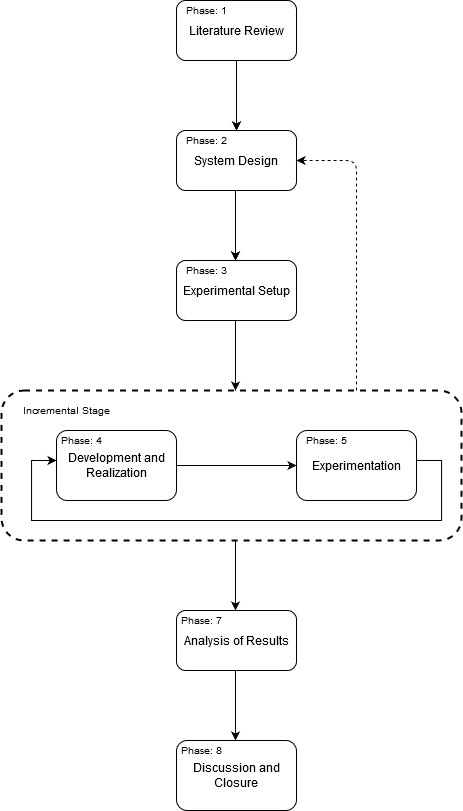
\includegraphics[width=0.5\textwidth]{figures/methodology/methodology}
	\caption{Methodology Flow Diagram}
	\label{fig:methodology_overview}
\end{figure}

The first phase constitutes a survey of the the relevant literature. During the second phase the identification and design of the modular subsystems takes place. This is followed by the third phase during which the modules are implemented according to their design.

In following the design paradigm of the spiral model, a feedback path from the development and realization stage back to the system design phase was incorporated. This was done to allow new information learned during the third phase to be incorporated into the system design.

Following the development and realization phase is an iterative stage which encapsulates both the experimental setup (phase 4) and the experimentation (phase 5).

During the seventh phase of the investigation the results are analysed and observations are recorded. The eighth phase concludes the investigation with a final discussion and closing remarks.


\section{Phase 1 - Literature}

During the first phase of the project, the relevant literature is reviewed. The objective of this phase is to determine the various techniques that have been established in the field of optical communication. For each of the topics a broad overview is presented, followed by a detailed review of specific concepts and theories.

The design and evaluation of a complex communication system involves reviewing theory in various areas and the following questions served as a guide for surveying the available literature.

%todo: consider improving these questions
\begin{itemize}
	%\item What are current examples of uni-directional communication systems?
	\item How might non-laser light be focused into a narrow beam? %Optics
	\item What properties make infrared light useful? %Optics
	\item What methods exist for detection of light? %Detection of Raditation
	\item What techniques exist for reliable communication? %Reliable Communication
	\item What techniques exist for the purpose of tone detection? %DSP &Analog processing
	%an item on filtering and pre-dsp stuff?
\end{itemize}

The literature review is presented in chapter \ref{ch_literature}.

%%%%%%%%%%%%%%%%%%%%

\section{Phase 2 - Design}

The design phase of this investigation is dedicated to the development of the individual modules and software algorithms. This phase begins with a decomposition of the uni-directional communication system into a set of modules. Figure \ref{fig:designoverview} provides a high-level overview of the system decomposition.

\begin{figure}[H]
	\centering
	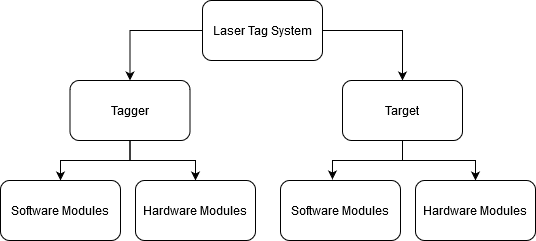
\includegraphics[width=0.7\linewidth]{figures/methodology/design_overview}
	\caption{Design Overview}
	\label{fig:designoverview}
\end{figure}

The second phase is documented in chapter \ref{ch_design}. For each module a brief description of the purpose and required functionality of the module is given. The design of module is then presented, including important calculations, circuit schematics and relevant diagrams where appropriate. For each module an image of the final implementation is also shown.

Throughout the design phase, various simulations were used to predict the behaviour of algorithms\footnote{Octave was used to validate algorithms} and circuits\footnote{LTSpice was used to simulate circuits}.

%%%%%%%%%%%%%%%%%%%%

\section{Phase 3 - Development and Realization}

The third phase concerns the development of the individual modules. During this phase each module was realized according its design.

Modules were first implemented on a breadboard to confirm valid behaviour. In the case of a failed implementation due to a design oversight the design was reworked, this is illustrated using a dotted feedback path from phase 3 to phase 2 in figure \ref{fig:methodology_overview}. Only the final module design and implementation has been documented in the body of this report.

With the exception of the STM32 development boards, all the module designs were implemented on strip-board. The use of PCB was avoided due to uncertainty caused by the COVID-19 epidemic.

%%%%%%%%%%%%%%%%%%%%


\section{Phase 4 - Experimental Setup}

The fourth phase is the experimental set-up. This phase outlines the procedure followed to setup the test and measurement equipment and the module or collection of modules for the purposes of performing experiments and gathering empirical data. Chapter \ref{ch_experimentation} is dedicated to the procedures followed for each experiment.

Due to the unique functionality of each module, it is necessary to use different experimental setups to evaluate different modules. Hence phase four forms part of an iterative stage which is used to illustrate that for various phases of experimentation, a unique experimental setup has been devised.

Equipment used throughout this investigation is documented at the end of this chapter in section \ref{sec:test_and_measurement_equipment}


%%%%%%%%%%%%%%%%%%%%



\section{Phase 5 - Experimentation}

Phase five concerns the execution of the experiments outlined in chapter \ref{ch_experimentation} and forms the second half of the iterative stage. During this phase, the experiments are executed and the results are prepared for analysis.

The objective of the experimentation phase is to provide results that may be used to gain insight into each module's performance. Results will consist primarily of empirical results, but in certain cases also include simulation results.

The results gathered during the experimentation phase are documented in chapter \ref{ch_results}.

%%%%%%%%%%%%%%%%%%%%

\section{Phase 7 - Analysis of Results}

The seventh phase of this investigation is the analysis of results gathered during the experimentation. The objective of this phase is to interoperate the results and draw insights.

During this phase, the performance of the individual modules is evaluated. Brief reasoning is provided where the results do not align with the theorised outcome.

%todo: confirm this is the structure
The analysis for each set of results has been place in chapter \ref{ch_results}. This has been done to increase readability.


%%%%%%%%%%%%%%%%%%%%

\section{Phase 8 - Discussion and Closure}

%todo: improve this section after completing phase 8
In this final phase of the project, the results and analysis of the results are discussed in the greater context of the research questions. The discussion will comment on the effectiveness of each of the modules. 

Discussion is bought to a close with a comment on the  proposals for further research.



%%%%%%%%%%%%%%%%%%%%

\section{Equipment}
\label{sec:test_and_measurement_equipment}
The following section outlines the equipment used during the development as well as test and measurement phases of the project.

\subsection{Oscilloscope and Function Generator}
To perform electrical measurements, the Picoscope 2205A by Pico Technology was used. The Picoscope has two input channels and a dedicated function generator. The function generator was used to inject waveforms in various experiments.

\subsection{Microcontroller Development}
The CubeIDE developer environment by STMicroelectronics was used to develop the firmware for the tagger, target and tone decoder's central processor.

\subsection{Signal Processing and Data Presentation}
The Octave mathematical programming language was used to develop and predict the behaviour of the digital signal processing algorithm as well as generate plots of the data collected in various experiments.

\subsection{Serial Communication}
Serial communication between the STM32 microcontrollers and personal computer were handled by Realterm \footnote{\url{https://sourceforge.net/projects/realterm/}}, a free serial monitor available for Windows.

\subsection{Circuit Simulation}
The LTSpice SPICE simulation environment by Linear Technology\footnote{LT corporation is owned by Analog Devices} was used to test and develop the circuit modules.

\subsection{Test and Measurement}
For general purpose measurements of voltages, current and resistance the Fragram T2612 digital multimeter was used.

The Sony Handycam DCR-HC26 video camera was used to \textit{see} the invisible beam spot produced by the LED focus system.

Measurements less than 300mm were performed using a digital caliper, measurements longer than 300mm we taken using a measuring tape.






